\documentclass[tikz,border=6pt]{standalone}
\usepackage[T1]{fontenc}\usepackage{helvet}\renewcommand{\familydefault}{\sfdefault}
\usetikzlibrary{arrows.meta,positioning,fit,backgrounds}
\begin{document}
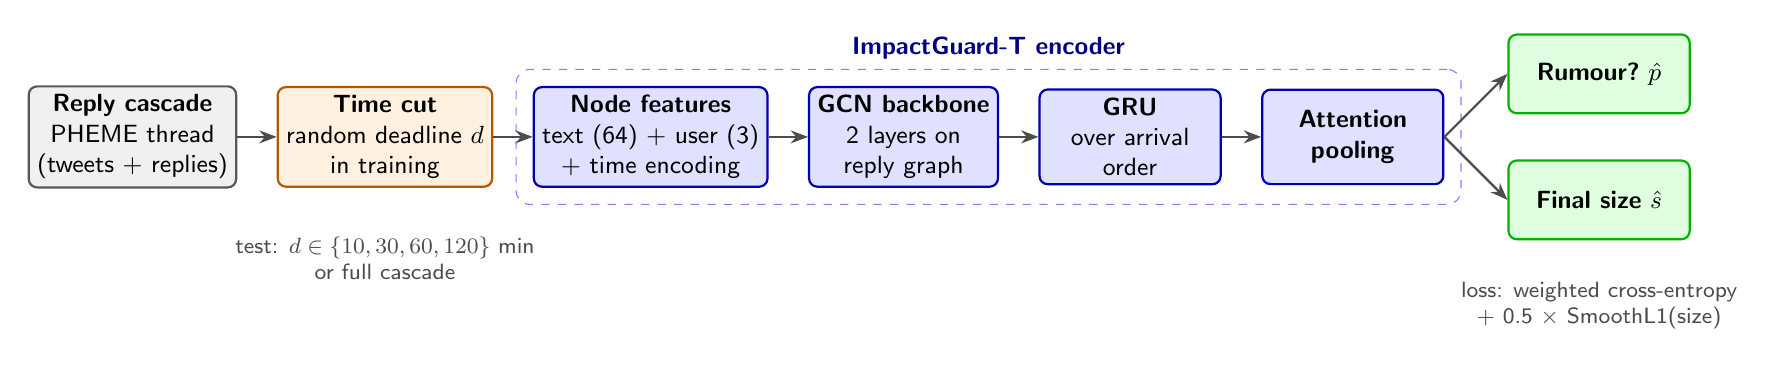
\begin{tikzpicture}[font=\small,node distance=5mm,
 b/.style={draw=#1!70!black,rounded corners=3pt,minimum height=12mm,minimum width=23mm,align=center,inner sep=3pt,fill=#1!12,thick},
 a/.style={-{Stealth[length=2.2mm]},thick,draw=black!70}]
\node[b=gray] (c) {\textbf{Reply cascade}\\PHEME thread\\(tweets + replies)};
\node[b=orange,right=of c] (t) {\textbf{Time cut}\\random deadline $d$\\in training};
\node[b=blue,right=of t] (e) {\textbf{Node features}\\text (64) + user (3)\\+ time encoding};
\node[b=blue,right=of e] (g) {\textbf{GCN backbone}\\2 layers on\\reply graph};
\node[b=blue,right=of g] (r) {\textbf{GRU}\\over arrival\\order};
\node[b=blue,right=of r] (p) {\textbf{Attention}\\\textbf{pooling}};
\node[b=green,right=8mm of p,yshift=8mm,minimum height=10mm] (h1) {\textbf{Rumour?}\ $\hat p$};
\node[b=green,right=8mm of p,yshift=-8mm,minimum height=10mm] (h2) {\textbf{Final size}\ $\hat s$};
\draw[a] (c)--(t);\draw[a] (t)--(e);\draw[a] (e)--(g);\draw[a] (g)--(r);\draw[a] (r)--(p);\draw[a] (p.east)--(h1.west);\draw[a] (p.east)--(h2.west);
\begin{scope}[on background layer]\node[draw=blue!50,dashed,rounded corners=5pt,fit=(e)(p),inner sep=6pt,label={[font=\small\bfseries,blue!50!black]above:ImpactGuard-T encoder}] {};\end{scope}
\node[below=4mm of h2,align=center,font=\footnotesize,text=black!70] {loss: weighted cross-entropy\\+ 0.5 $\times$ SmoothL1(size)};
\node[below=5mm of t,align=center,font=\footnotesize,text=black!70] {test: $d\in\{10,30,60,120\}$ min\\or full cascade};
\end{tikzpicture}
\end{document}
